% Template; to be used with:
%          spconf.sty  - ICASSP/ICIP LaTeX style file, and
%          IEEEbib.bst - IEEE bibliography style file.
% --------------------------------------------------------------------------
\documentclass{article}
\usepackage{spconf,amsmath,graphicx}

% Example definitions.
% --------------------
\def\x{{\mathbf x}}
\def\L{{\cal L}}

% Title.
% ------
\title{A Vision-Based Intelligent System for Eye Clinic Automation}
%
% Single address.
% ---------------
\name{Lim Chang Siang,  Li Zhenghao Kelvin, Zhong Xiaohui, Zheng Xiaolan}
\address{Institute of Systems Science, National University of Singapore, Singapore 119615}

\begin{document}
%\ninept
%
\maketitle
%

\begin{abstract}

Vision loss poses a significant health risk, particularly in aging populations. It is closely linked to reduced quality of life, increased dependence, and worsened health outcomes. Timely detection and treatment can help delay the progression of vision loss. However, regular eye checks often face accessibility challenges due to the scarcity of trained specialists. To address this issue, our project aims to enhance the accessibility of routine eye health assessments by developing a vision intelligent system to enable automating visual acuity checks. By leveraging technology, we aspire to improve the availability and convenience of such assessments, ultimately promoting proactive eye care. 

\end{abstract}
%

\begin{keywords}
machine vision, medical, automation, ophthalmology,
\end{keywords}
%
\section{Introduction}
\label{sec:intro}
Sight is often considered the sense that is most important and valued \cite{enoch2019evaluating}. However, accurate measurement of a person’s vision is difficult. This is not only because it is subjective, but also that vision itself has many facets. One of the universally used measure of vision is the visual acuity test.

Visual acuity is a core component of the eye examination. It provides the tester an objective measurement of the subject’s vision. This is usually done via a reading off a visual acuity chart, while covering one eye at a time \cite{dejong2022history}. In this project, we aim to design a vision system to be able to detect a patient’s pose during visual acuity examination. In particular, whether or not patients are wearing glasses, and whether the occlude is correctly positioned and used.

Accurate measurement of a person’s vision is difficult. This is not only because it is subjective, but also that vision itself has many facets. One of the universally used measure of vision is the visual acuity test \cite{dejong2022history}. 

The visual acuity test consists of a display showing varying sizes of letters or characters, called optotypes (Figure \ref{optotype}), usually arranged in a vertical fashion in decreasing order of size. Patients are instructed to read, with each eye singly, till the smallest letter that they can see. For patients who require glasses to read, we would instruct the patients to read with their glasses on.
\begin{figure}[tbh]
    \begin{center}
        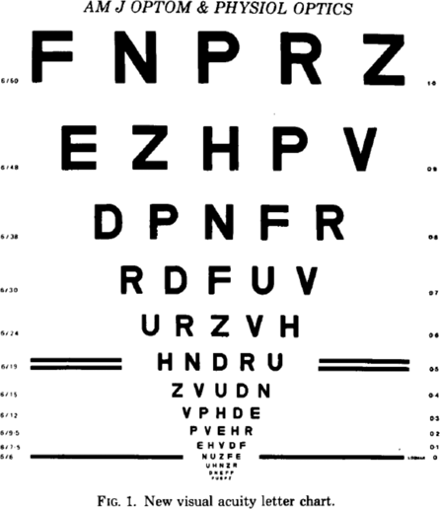
\includegraphics[width=3cm]{optotype.png}\
        \caption{Example of optotype used during visual acuity testing.\label{optotype}} 
    \end{center}

\end{figure}

To ensure that the patients are using one eye in turn, they are instructed to hold an occlude (Figure \ref{occluder}) to cover the fellow eye. Some versions of the occluder have an additional pinhole segment to reduce the effect of refractive error.
\begin{figure}[tbh]
    \begin{center}
        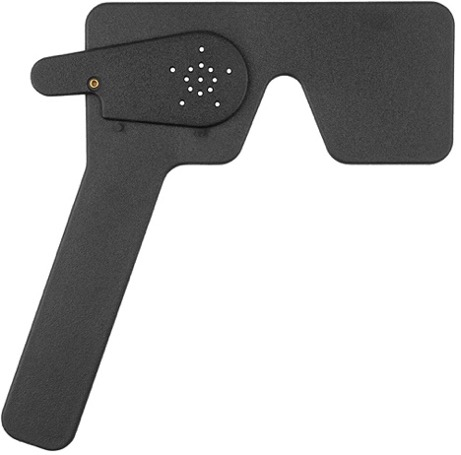
\includegraphics[width=3cm]{occuluder.jpg}\
        \caption{Occluder with pinhole. \label{occluder}} 
    \end{center}
\end{figure}
\section{Literature review}
Visual acuity test is based on a rule-based scorecard to provide an objective information about the person's vision health. The rule-based nature of the task makes it an attractive candidate for automation.

\subsection{Related research works}
According to the World Health Organization (WHO), there are over 2.2 billion people worldwide with varying degrees of vision impairment. It is estimated that at least half of these cases can be prevented through early screening and detection \cite{who_blindness}. One effective examination method is the visual acuity check, traditionally performed in optician or specialist clinics by trained professionals. However, this approach limits scalability, especially considering the increasing needs of an aging population. To address this emerging demand, several groups have explored the feasibility of digitalizing the Visual Acuity (VA) check, allowing easy access via smartphones.

EyeChartPro, for example, has developed an iPad application that enables patients to self-check their vision at home \cite{zhang2023pilot}. Although this study found that the iPad display method is as accurate as the traditional lightbox method for individuals with 20/20 vision, it showed greater variation for those with visual impairments. In another study, researchers developed the "V@Home" application, which allows patients to autonomously perform VA checks at home using their iPhones. The application includes audio analysis using Mel-frequency cepstral coefficient (MFCC) to analyze speech and provide automatic test results. Users receive instructions from the application to conduct the test. Evaluation of this application demonstrated high reliability and accuracy compared to routine care \cite{han2019development}.

These works collectively demonstrate the potential for scaling the VA test through digitalization. However, it is worth noting that these studies were conducted in controlled environments, and concerns have been raised about ensuring patients follow the test guidelines and do not attempt to manipulate the results \cite{zhang2023pilot}. To the best of our knowledge, there is currently no digital VA application with patient monitoring capabilities to automatically observe patient actions, provide feedback, and offer suggestions for correction in real-world implementations.

\subsection{Related commercial solutions}
In the realm of self-check systems for visual acuity (VA), there exists at least one commercially available product. In 2008, a start-up called SoloHealth introduced a product called EyeSite, which is a standalone booth enabling individuals to assess their vision health. The pilot trial of this product involved testing 15,000 individuals over a span of 5 weeks. Notably, 25\% of participants had never undergone an eye exam before, indicating the potential accessibility of self-test kiosks, particularly for individuals facing significant barriers to visiting a doctor's clinic \cite{uspharmacist_website}. 

\section{System Requirements}
In this study, we have selected Tan Tock Seng Hospital (TTSH) as our case study, specifically focusing on the Ophthalmology Specialist Outpatient Clinic (SOC) located in Singapore. To gain valuable insights, we conducted interviews with clinical experts in the field. Through these interviews, we were able to identify four key requirements that aim to address the challenges faced by the clinic and alleviate their pain points (Figure \ref{system-requirement}).

\begin{itemize}
\item Ability to confirm the person's identity through their identification document.
\item Ability to confirm that the examination room has only one person present.
\item Ability to determine if the person is wearing glasses or not.
\item Ability to determine which eyes (left or right) is occuluded using the occuluder tool. 
\end{itemize}

\begin{figure}[tbh]
    \begin{center}
        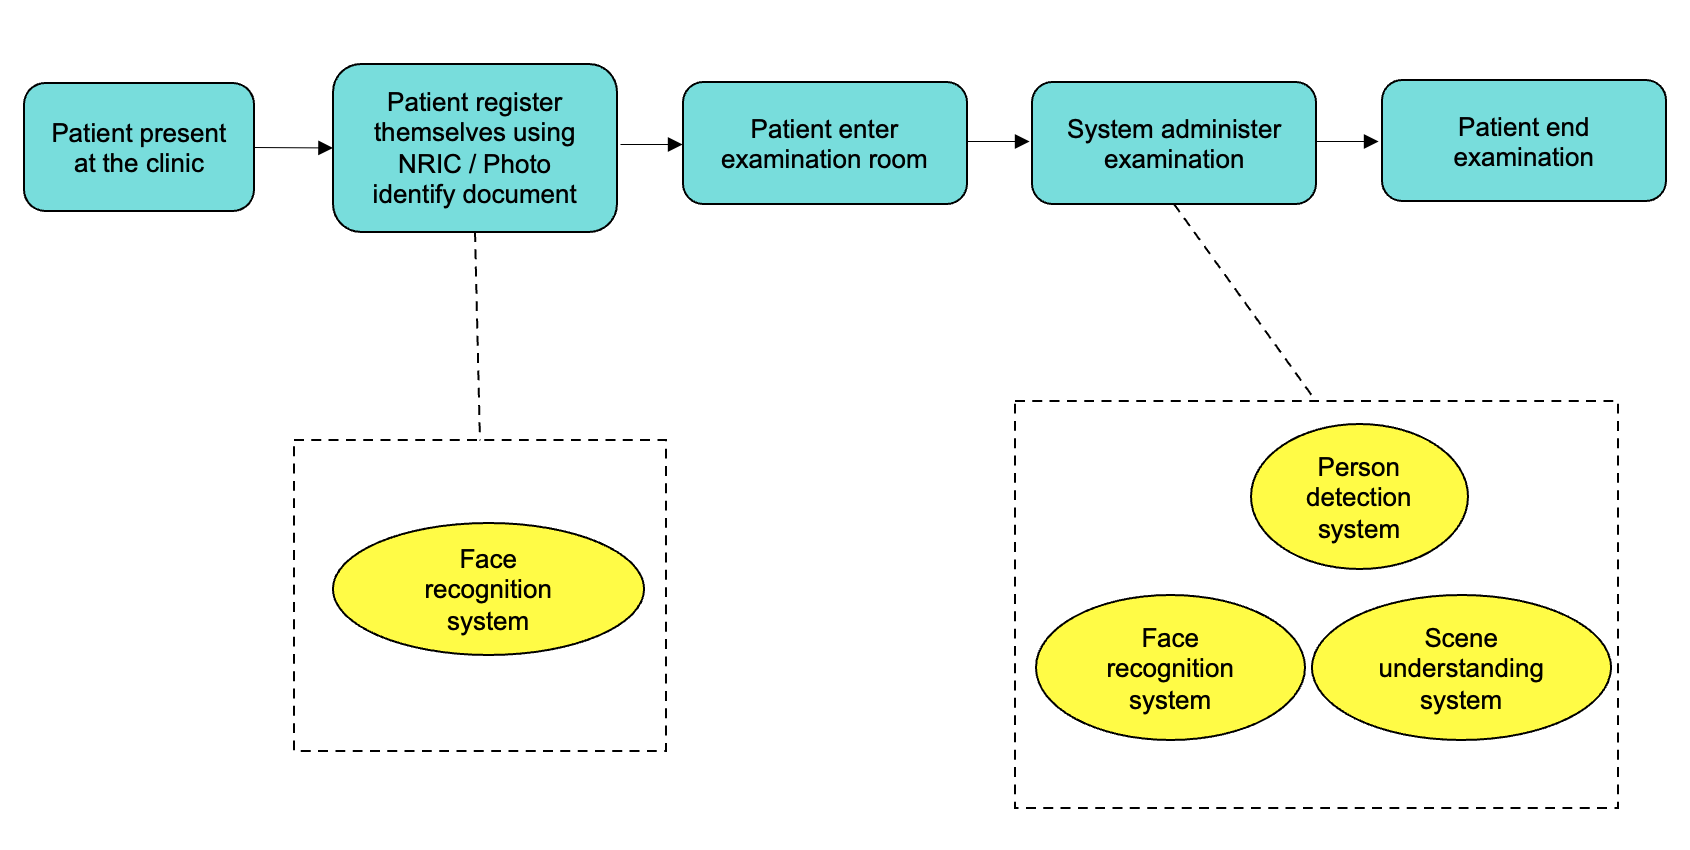
\includegraphics[width=8cm]{solution-overview.png}\
        \caption{Overview of system requirement \label{system-requirement}} 
    \end{center}
\end{figure}

Based on the requirements, we proposed to develop 3 vision intelligent systems, namely,

\begin{itemize}
\item Face Recognition System: Confirm that the right patient is receiving care
\item Person Detection: To ensure that there is only one person present for the examination
\item Scene Understanding System: To provide context and interpretation on the patient actions
\end{itemize}

\section{Proposed approach}
\subsection{Person Recognition System}
\begin{figure}[tbh]
    \begin{center}
        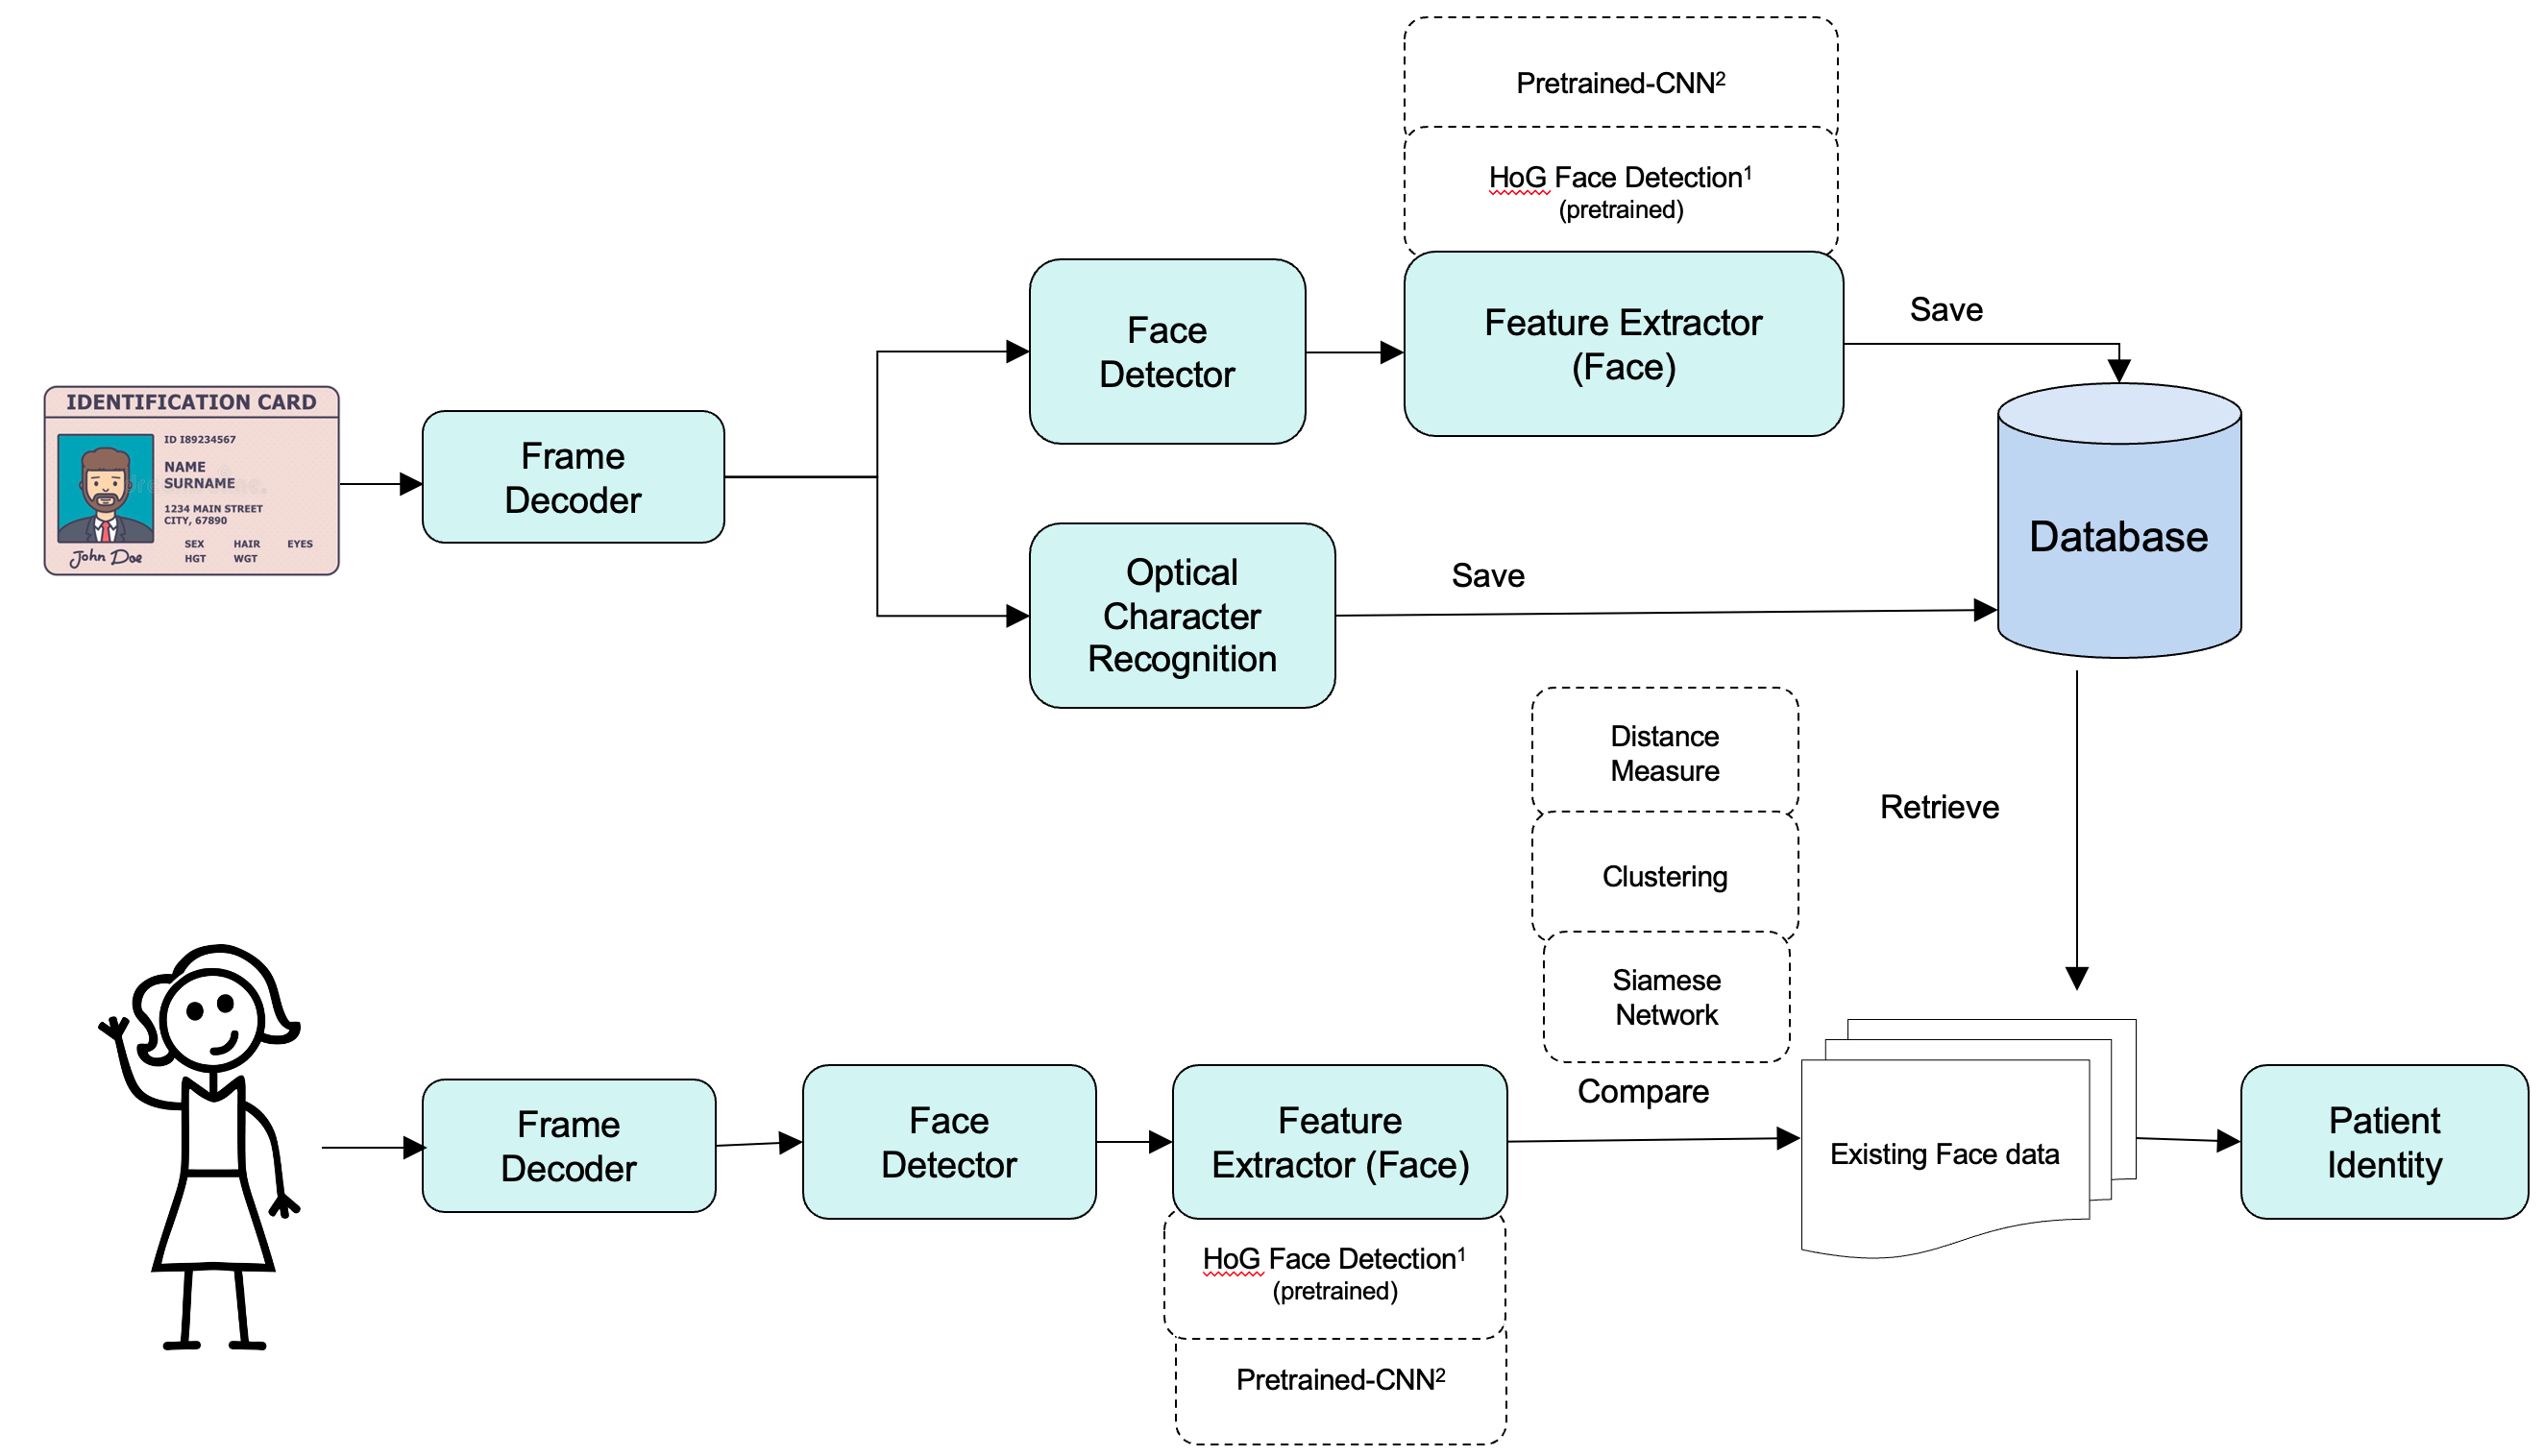
\includegraphics[width=8cm]{person-recong.png}\
        \caption{Approach for Person Recognition System \label{figure2}} 
    \end{center}
\end{figure}
The person recognition system is used for 2 purposes:
\begin{itemize}
    \item Patient Registration: The person recognition system is designed to register patients into the identity database by utilizing information from their National Identity Registration Card (NRIC). The system will effectively identify the portrait photo, detect the person's name, extract the facial features from the portrait, and securely store them within the database.
    \item Patient Re-identification: The system will accurately identify the person present in the scene, crop their face, extract the facial features, and utilize a gallery method to identify the closest matched identity for re-identification purposes.
\end{itemize}
In order to extract facial features, we employed a combination of techniques, including the use of Histogram of Gradient (HoG) and various Convolutional Neural Network (CNN) feature extractors. To compare two face images, we utilized multiple methods, such as cosine and Euclidean distance measures, as well as a Siamese network, to determine the most effective approach.

To extract the name information from an image, we utilized an established Optical Character Recognition solution (Tesseract) to extract the text. Additionally, we employed a rule-based approach to accurately determine the name string.

\subsection{Person Detection}
\begin{figure}[tbh]
    \begin{center}
        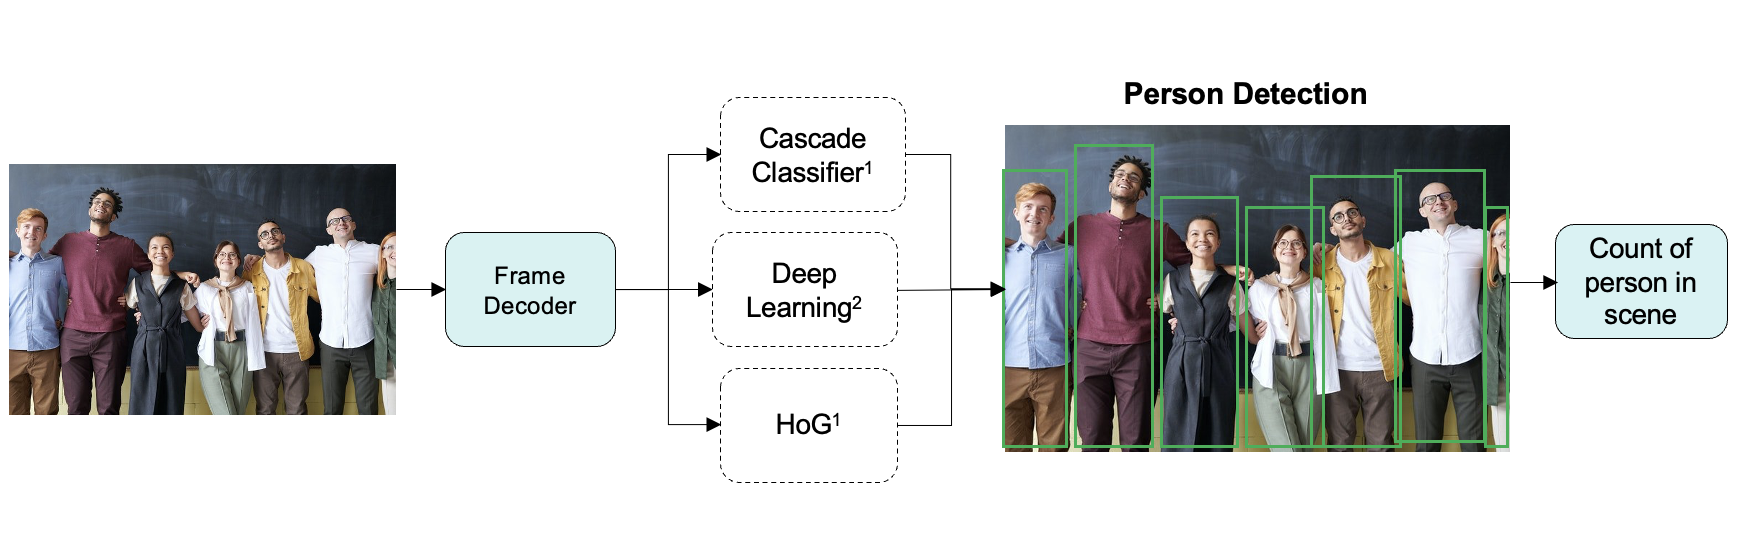
\includegraphics[width=8cm]{person-detection.png}\
        \caption{Approach for Person Detection System \label{figure2}} 
    \end{center}
\end{figure}

The use case for person detection is to count the number of human person present in the scene and report the number accordingly for downstream usage. For our solution, we intend to experiment both machine learning and deep learning approaches, including using Cascade Classifier, Histogram of Gradient (HoG) and existing Deep Learning model. Training of a custom cacasde classifier model require huge amount of data and computational power, we intend to first explore the feasibility of existing models for our purpose.
\subsection{Scene Understanding System}
\begin{figure}[tbh]
    \begin{center}
        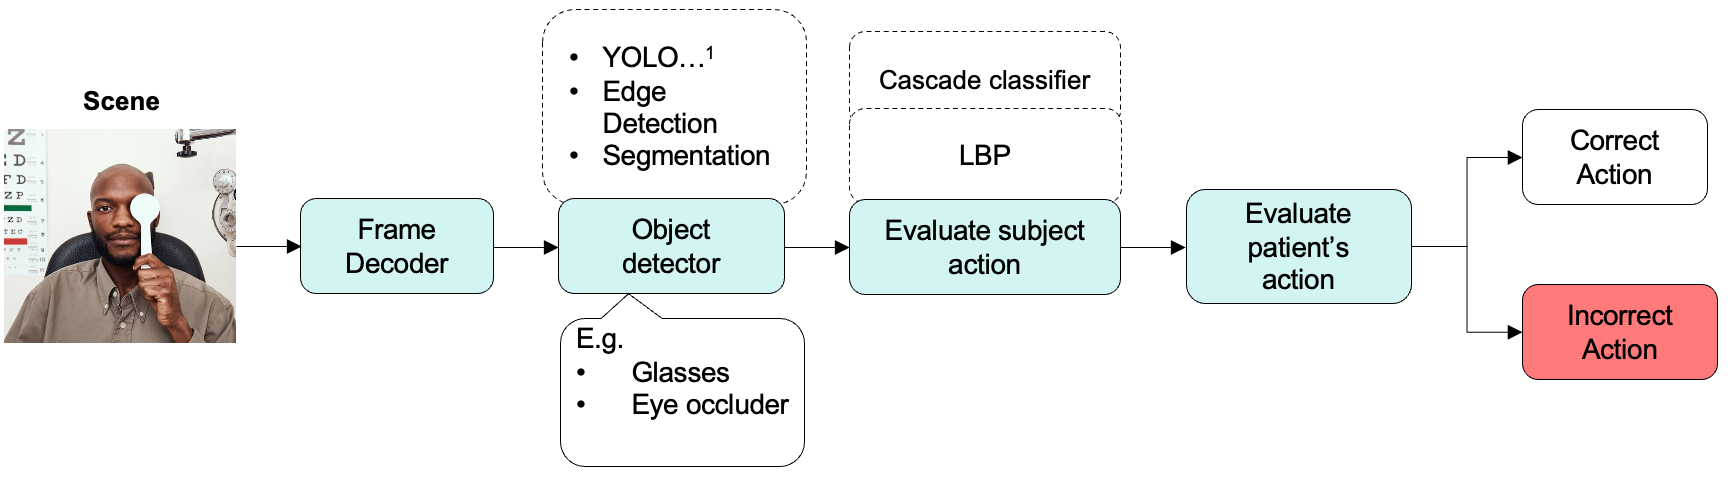
\includegraphics[width=8cm]{scene-understanding-2.png}\
        \caption{Approach for Scene Understanding System\label{figure2}} 
    \end{center}
\end{figure}
The purpose of scene understanding system is to able to identify the scene with person into the following categories:
\begin{itemize}
    \item Wearing Glasses
    \item Not Wearing Glasses
    \item Occulude Left Eye
    \item Ouuclde Left Eye with Pinhole on Right Eye
    \item Occulude Right Eye
    \item Occulide Right Eye with Pinhole on Left Eye
\end{itemize}
The identification of eye occlusion actions can be accomplished by detecting the presence of an "occluder" tool within the scene. To achieve this, we will explore a range of image processing techniques such as edge detection and segmentation, complemented by the implementation of modern object detection techniques like You Only Look Once (YOLO) \cite{redmon2016yolo}. These approaches will enable us to detect the object and ascertain the specific type of action occurring in the scene.

\section{Dataset}
To develop the person recognition system and person detection system, we utilized the Labelled Face in the Wild dataset, a publicly available resource \cite{lfwTech}. Employing the scikit-learn package, we configured the parameters to exclusively include classes with a minimum of 100 available images. Consequently, we acquired a total of 1140 facial images representing 5 distinct person classes.

For the scene understanding system, we encountered a challenge as there were no readily available curated open-source datasets specifically designed for individuals wearing eye occluders. Therefore, in order to proceed with this particular project module, we took the initiative to create our own dataset. To ensure ethical compliance and patient privacy, the dataset collection process was conducted at the Tan Tock Seng Hospital Eye Clinic, with the assistance of volunteers, specifically administrative personnel. This approach allowed us to gather the necessary data while upholding the highest ethical standards.

All images were taken in a brightly lit indoor environment against a plain backdrop. Participants all had to wear masks as part of hospital policy. This is also important as the system is intended to be deployed in a clinical setting and it’s expected that the end-users will be wearing masks. We also collected images of participants who wore spectacles and participants without spectacles. This will also be representative of the population for which this system is intended for.

All images were captured using an Apple iPhone 11 camera (Cupertino, California, United States). The images were taken in portrait mode, at a resolution of 3024 x 4032 pixels, in RGB mode. Files were saved as .jpeg format in the database.

A total of 40 images were collected from 10 participants in 4 poses, this translates to 4 classes, each with 10 instances. These were taken consecutively and on the same day. The 4 poses are (1) right eye occluded without pinhole (2) left eye occluded without pinhole (3) right eye occluded with pinhole (4) left eye occluded with pinhole.

 \begin{figure}[tbh]
    \begin{center}
        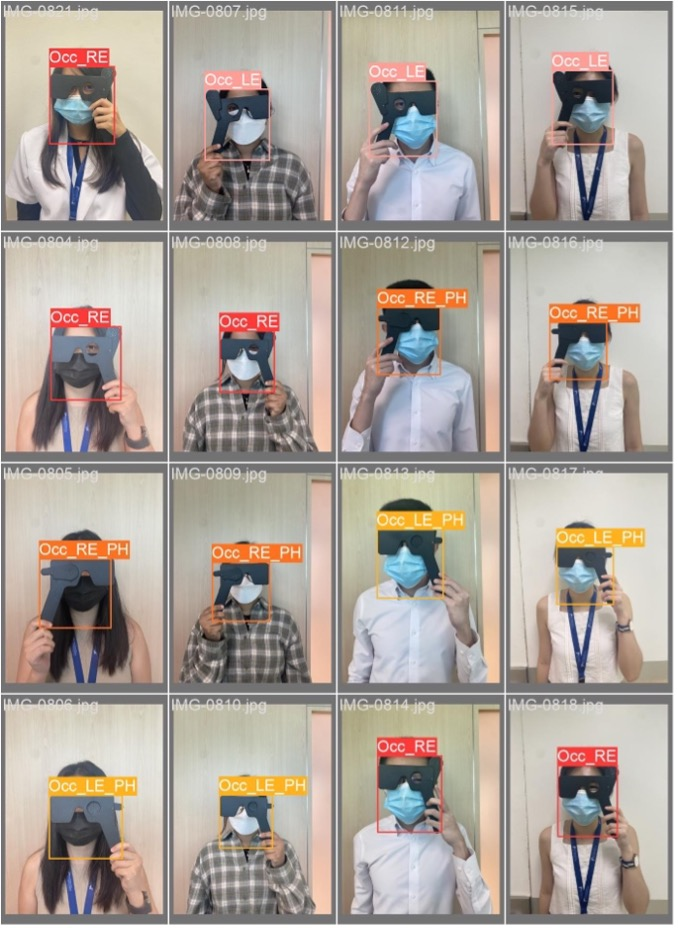
\includegraphics[width=8cm]{yolo_annotated.jpg}\
        \caption{Samples of person with occuluder images with human annotation using Roboflow \cite{roboflow}
        \label{figure7}} 
    \end{center}
\end{figure}

Using images collected from volunteers, we employed an unsupervised segmentation tool called the Segment Anything Model (SAM) to generate segmentation masks for various objects present in the scene. From a dataset comprising 40 images, we successfully created a total of 1153 masks. Among these, 1092 masks corresponded to the "others" category, while 15 masks were classified as "left," 18 as "left\_pinhole," 13 as "right," and 14 as "right\_pinhole" (Figure \ref{sam-mask}). Since the dataset exhibited significant class imbalance, we performed oversampling on the underrepresented classes. Consequently, we obtained a final dataset comprising 5460 masks, with 1092 images allocated to each of the 5 classes (Figure \ref{data-resampling}).

 \begin{figure}[tbh]
    \begin{center}
        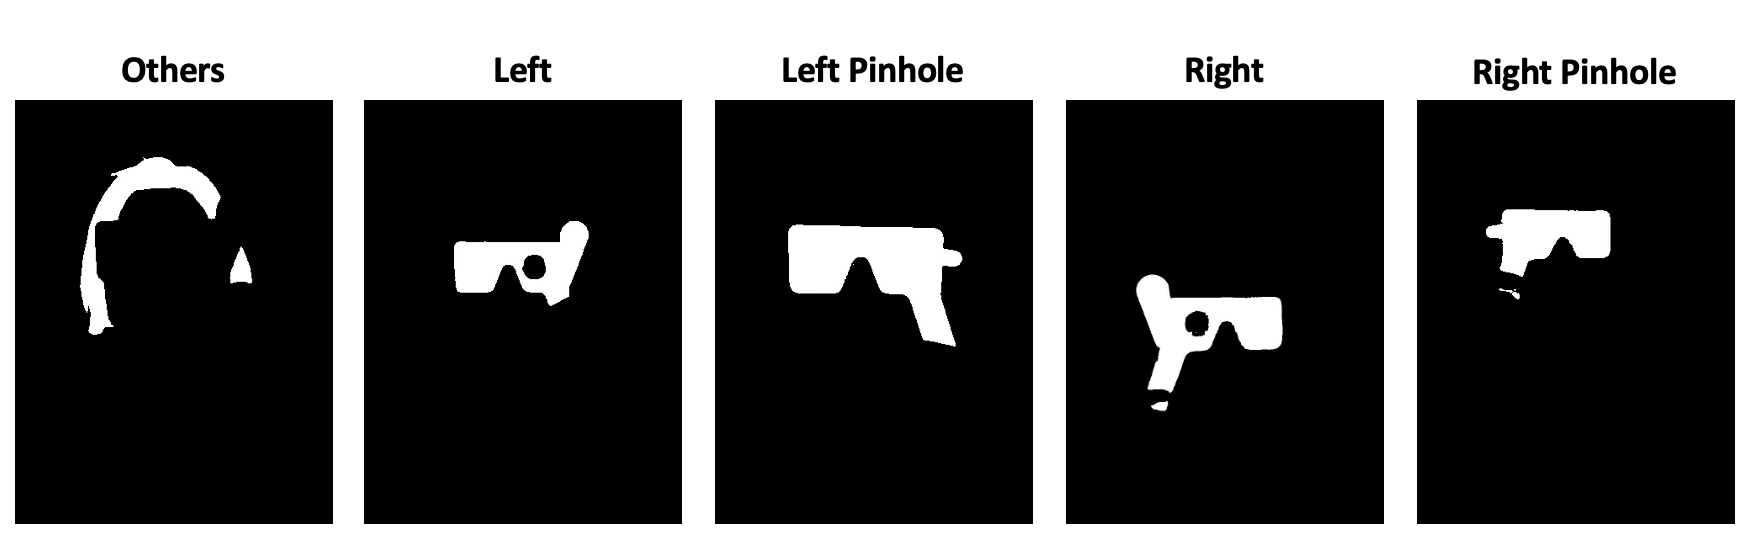
\includegraphics[width=8cm]{mask-example.png}\
        \caption{Masks generated using Segment Anything Model \label{sam-mask}} 
    \end{center}
\end{figure}


\begin{figure}[tbh]
    \centerline{\begin{tabular}{cc}
        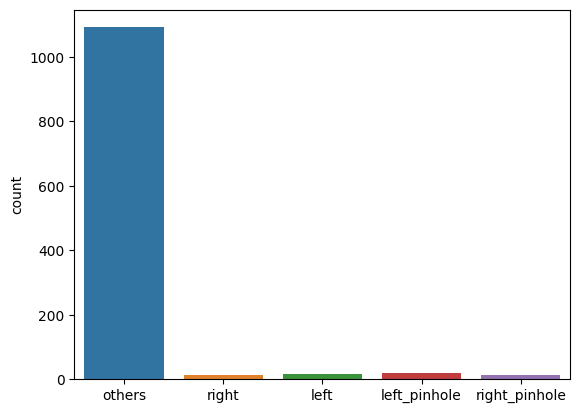
\includegraphics[width=3.5cm]{mask_stats.png}
        &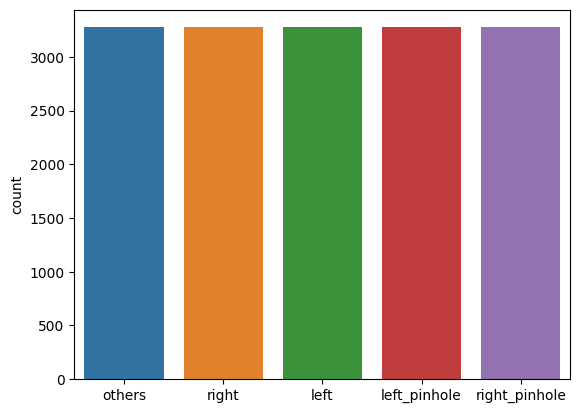
\includegraphics[width=3.5cm]{mask_stat_balanced.png}\\
    (a) & (b)
    \end{tabular}}
    \caption{(a) Original Dataset, (b) Balanced using resampling approach.\label{data-resampling}}
\end{figure}

\section{Experimental results}
\subsection{Person Recognition System}
In our person recognition system, we employed various feature extraction techniques for human face images. These techniques encompassed Histogram of Gradient (HoG), ResNet50, VGG19, VGGFace, and a customized CNN model trained using a Siamese network (Figure \ref{siamese-network}). To train our custom CNN model, we utilized 3380 pairs of images and evaluated its performance on 850 pairs of images. To ensure efficiency, we implemented an early stopping rule, terminating training if there was no improvement in accuracy after 10 epochs.

\begin{figure}[tbh]
\begin{center}
    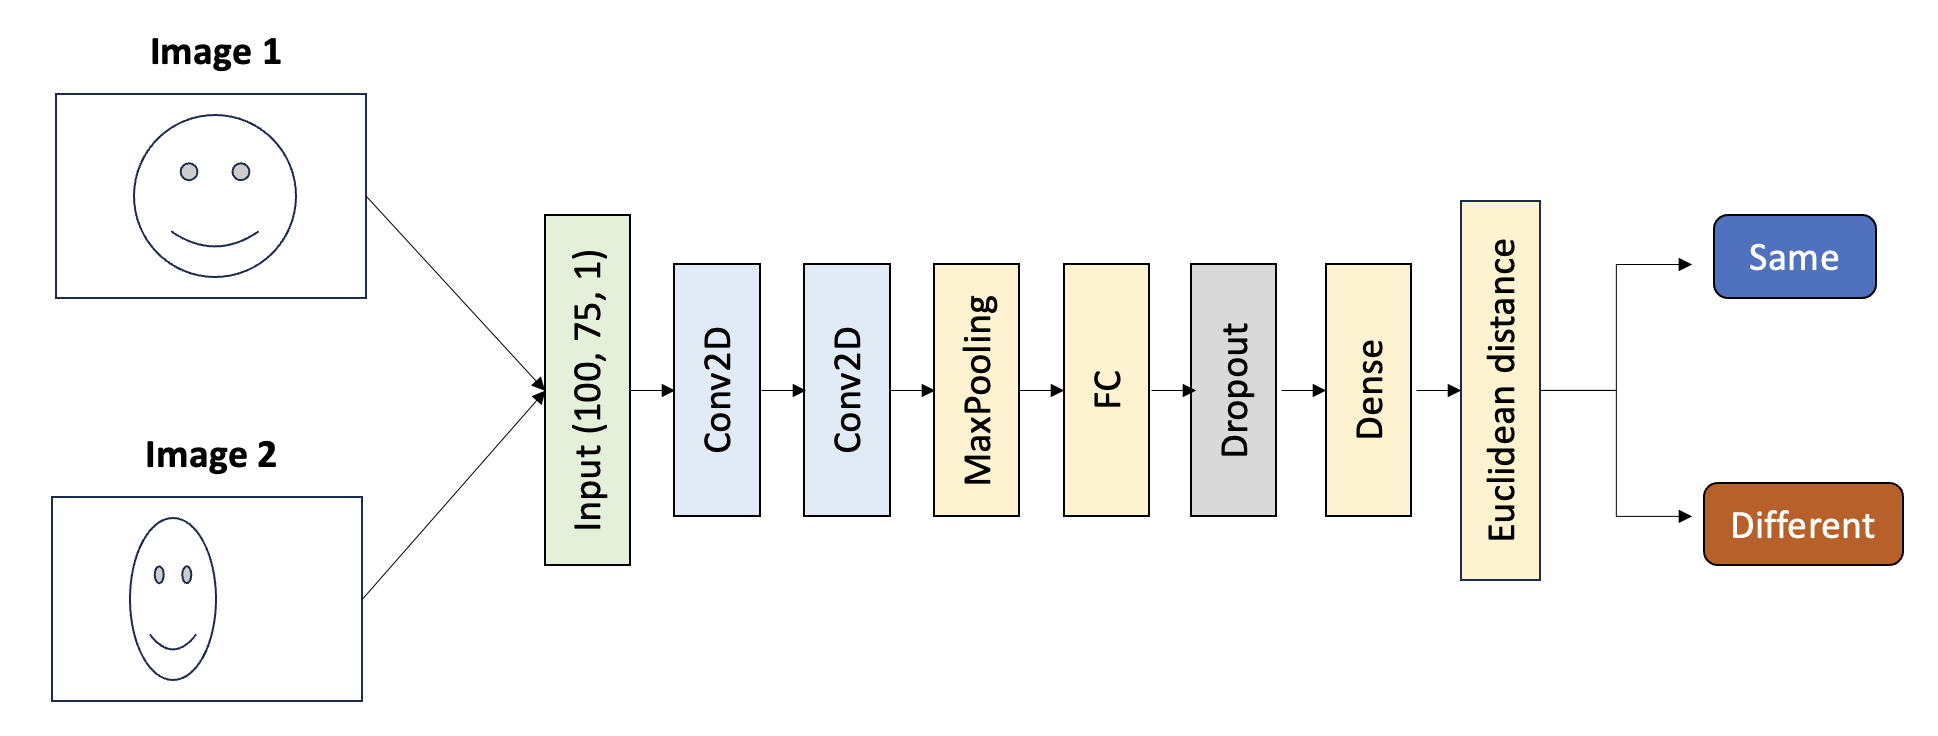
\includegraphics[width=9cm]{siamese-training.png}
    \caption{Siamese model architecture\label{siamese-network}}
\end{center}
\end{figure}

\begin{table}[tbh]
\caption{Performance comparison for Person Recognition System.}\label{table1} \centerline{
    \begin{tabular}{c|c|c}
    \hline\hline
    Approach & Distance Measure & Accuracy \\
    \hline\hline
    HoG & Cosine Similiarity & $0.4647$ 
    \\\hline
    HoG & Euclidean Distance & $0.4647$ 
    \\\hline
    ResNet50 & Euclidean Distance & $0.5017$
    \\\hline
    VGG19 & Euclidean Distance & $0.3160$
    \\\hline
    VGGFace & Euclidean Distance & $0.6690$
    \\\hline
    Custom CNN & Euclidean Distance & $0.1101$
    \end{tabular}
    }
\end{table}

For ResNet50 and VGG19, we utilized pre-trained weights from the ImageNet dataset \cite{imagenet_cvpr09} to perform feature extraction. VGGFace, renowned for facial recognition, was trained on human face images using the VGG19 architecture \cite{parkhi2015deep}. Our training process involved employing the Labeled Face in the Wild (LFW) dataset \cite{lfwTech}, and we evaluated the model's accuracy in correctly identifying image pairs.

\begin{figure}[tbh]
    \begin{center}
        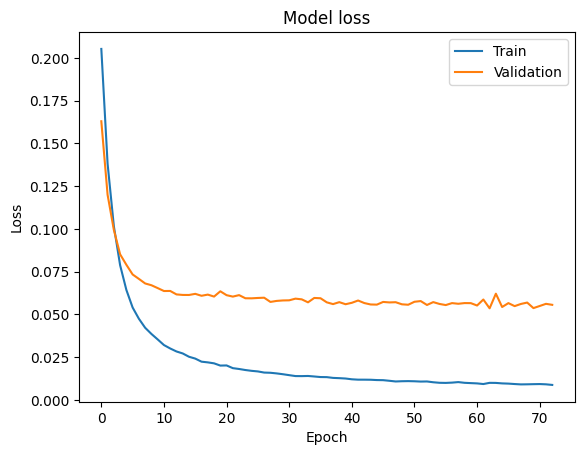
\includegraphics[width=6cm]{simese-network-training-loss.png}\
        \caption{Training loss with Siamese Network after 70 epoch\label{figure2}} 
    \end{center}
\end{figure}

\begin{figure}[tbh]
    \begin{center}
        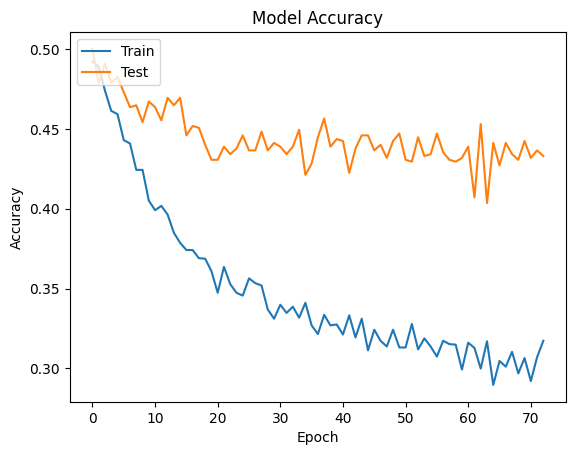
\includegraphics[width=6cm]{simense-network-training-acc.png}\
        \caption{Accuracy with Siamese Network after 70 epoch\label{figure2}} 
    \end{center}
\end{figure}

Table 1 summarises the result of our experiment. Using HoG feature vector, we found no difference in using either Cosine similarity or Euclidean distance measure. As such, we decide to stick to only using Euclidean distance measure. In our evaluation, we found that VGGFace has the best accuracy performance of 67\%, while our custom CNN model has the lowest score of 11\% (Table 1). 
\subsection{Face Detection System}
In our solution, face detection plays a crucial role in the following tasks:

\begin{enumerate}
  \item Identifying individuals and confirming their identity against registered information.
  \item Counting the number of people present in the scene, ensuring only one person is detected.
\end{enumerate}

There are several face detection methods available, including:
\begin{itemize}
    \item CNN
    \item Eigenfaces
    \item Fisherfaces
    \item Haar Cascade
\end{itemize}
Among these methods, we selected Haar Cascade due to its ease of deployment and fast detection capabilities.

The Haar Cascade algorithm is implemented through the \texttt{CascadeClassifier} class provided by the OpenCV library. This algorithm is based on the Viola-Jones algorithm, which is widely recognized for its efficiency in object detection, including face detection.

The method described above has certain limitations and challenges. To assess its reliability, several experiments were conducted, including variations in face angles and movement.

It was observed that this model is capable of detecting faces within a certain range of angles. However, when the face moves rapidly, the bounding box may not accurately display the face's actual location. In real-world scenarios, patients are typically instructed to minimize fast movements and face the camera directly, mitigating this issue.

Another factor tested was the presence of occlusion on the face. The model performed well in detecting faces with occlusion covering a substantial portion of the face. However, if the coverage is less than half, the accuracy of detection may be compromised.

Furthermore, the model demonstrated effectiveness under different lighting conditions, including both weak and bright light environments. Nevertheless, in practical scenarios, it is advisable to ensure sufficient brightness for optimal performance.

These experiments shed light on the strengths and limitations of the face detection method, providing insights for its application in real-world scenarios.

The \texttt{CascadeClassifier} utilizes a cascade of weak classifiers, which are simple and computationally efficient classifiers. These weak classifiers are combined to form a strong classifier capable of effectively detecting the target object.

\begin{figure}[tbh]
    \begin{center}
        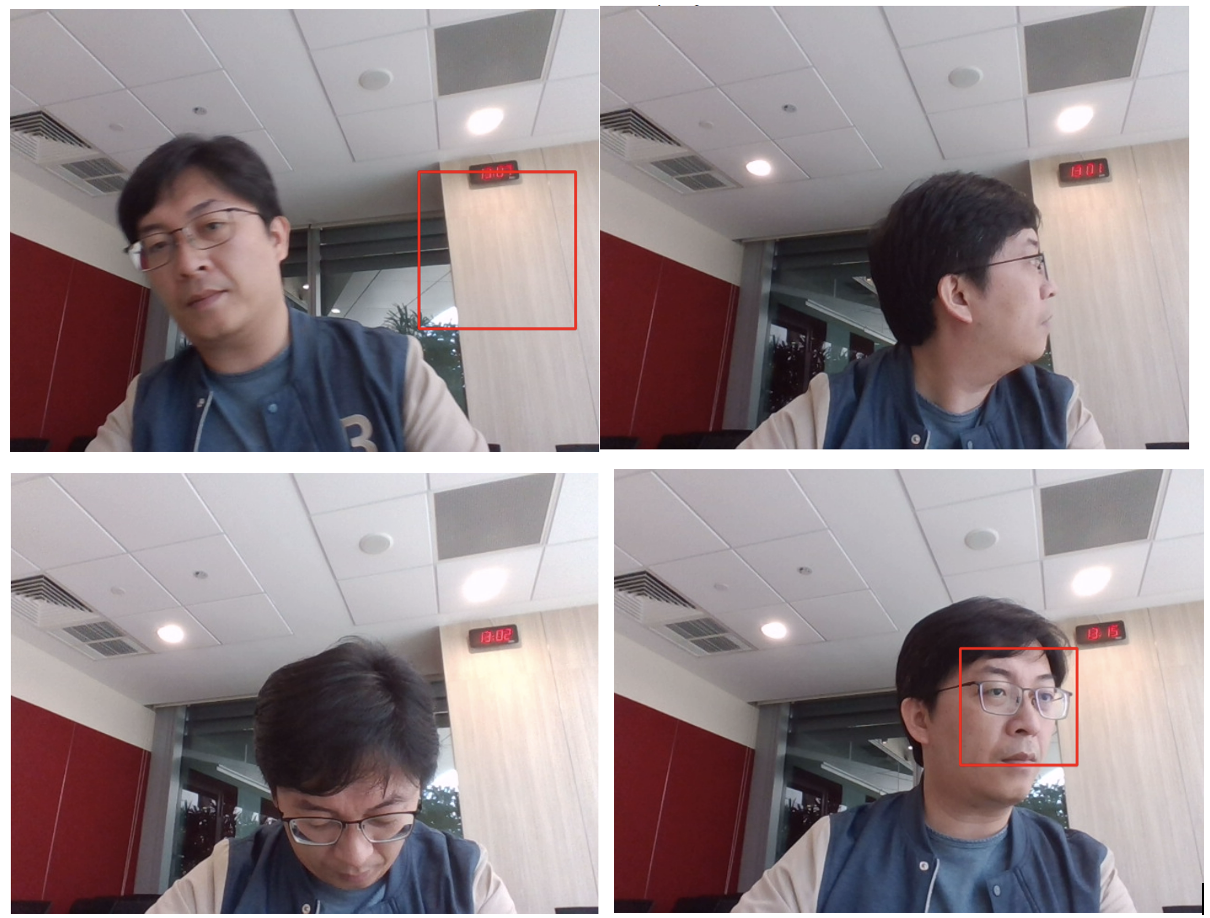
\includegraphics[width=8cm]{face-detection-test-one.png}\
        \caption{Different angles of the face and movement\label{figure2}} 
    \end{center}
\end{figure}

\begin{figure}[tbh]
    \begin{center}
        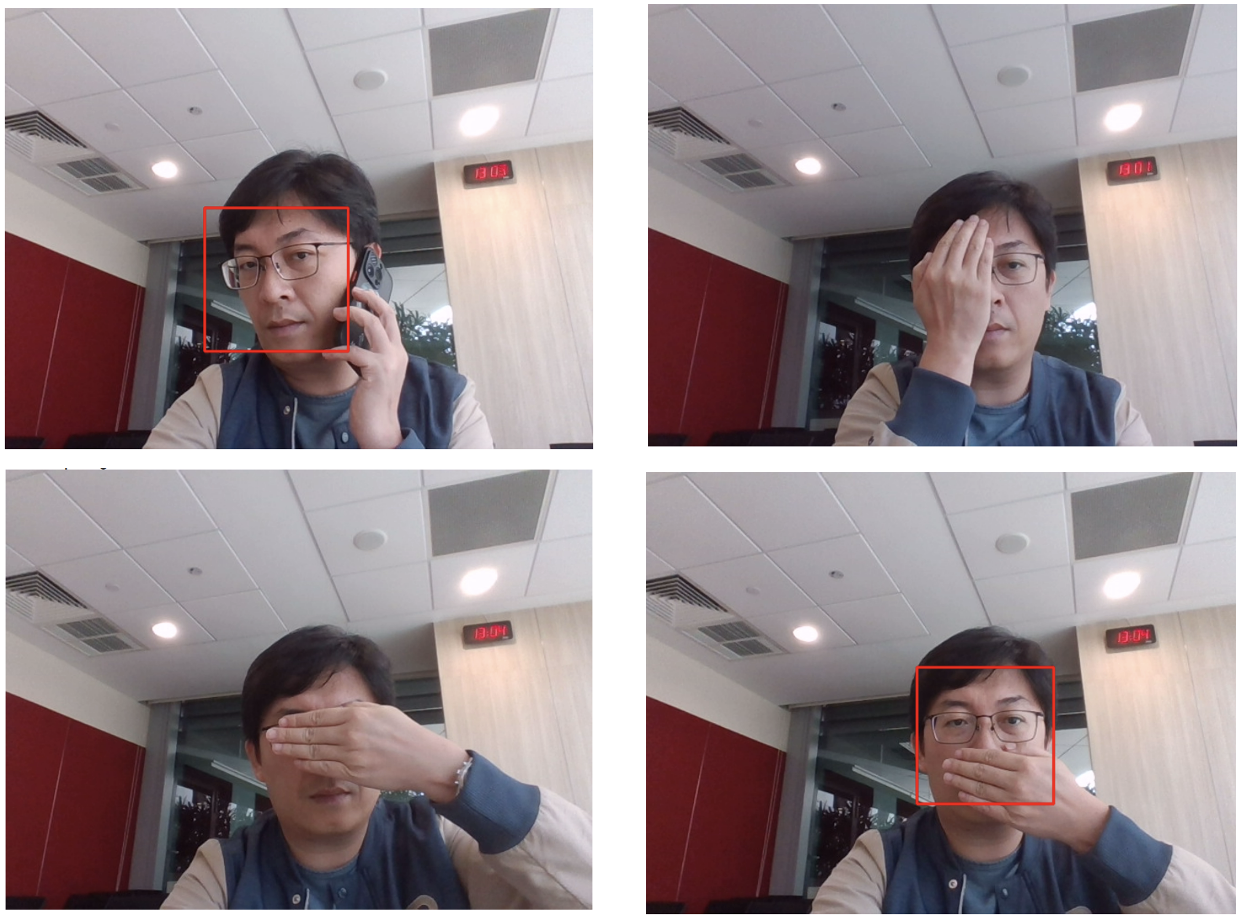
\includegraphics[width=8cm]{face-detection-test-two.png}\
        \caption{2)	Occlusion of face\label{figure2}} 
    \end{center}
\end{figure}

\begin{figure}[tbh]
    \begin{center}
        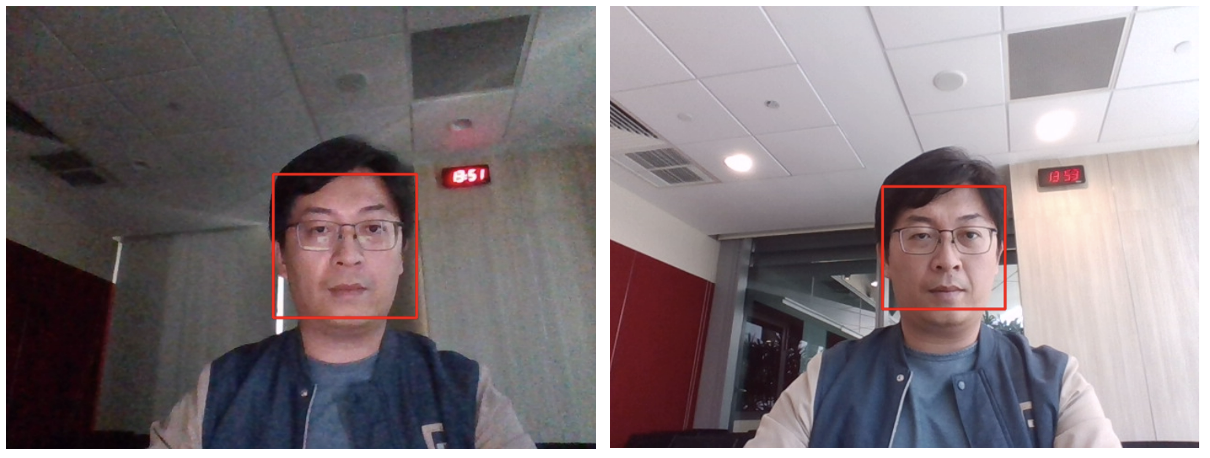
\includegraphics[width=8cm]{face-detection-test-three.png}\
        \caption{3)	Different lighting condition\label{figure2}} 
    \end{center}
\end{figure}

\subsection{Scene Understanding System}
In our scene understanding system, the glasses detection function plays a crucial role in verifying the patient's status before conducting the acuity test. In this project, we have explored hand-crafted techniques to detect the presence of glasses.

The traditional approach we employed focuses on examining the presence of a glasses bridge across the nose area. By determining the presence or absence of a bridge, we can deduce whether glasses are worn by the patient.

To begin, we locate the nose area of individuals using face landmark detection. This technique involves identifying and tracking key points on a person's face. Over time, the advancement of this technique has expanded the number of key points from a mere five to several hundred. In our project, we utilized the widely-used 68 key points face landmarks. To do this, we obtained a pre-existing .dat landmark file containing the information for these 68 points.

Within the 68-point landmark, the nose area is represented by points 28 to 31. We utilized the Dlib face detection model to acquire all 68 facial landmarks. Subsequently, we applied Gaussian blur and Canny edge detection to generate an edge profile for the area of interest. By examining the edge detection results, we can identify the profile of a glasses bridge, if present.

The final step involves determining the presence of glasses. We draw a vertical line across the nose area and analyze if any white-colored pixels are detected. The presence of white color signifies the existence of a glasses bridge, thus confirming the presence of glasses on the nose. Conversely, the absence of white color indicates the absence of glasses.

\begin{figure}[tbh]
    \begin{center}
        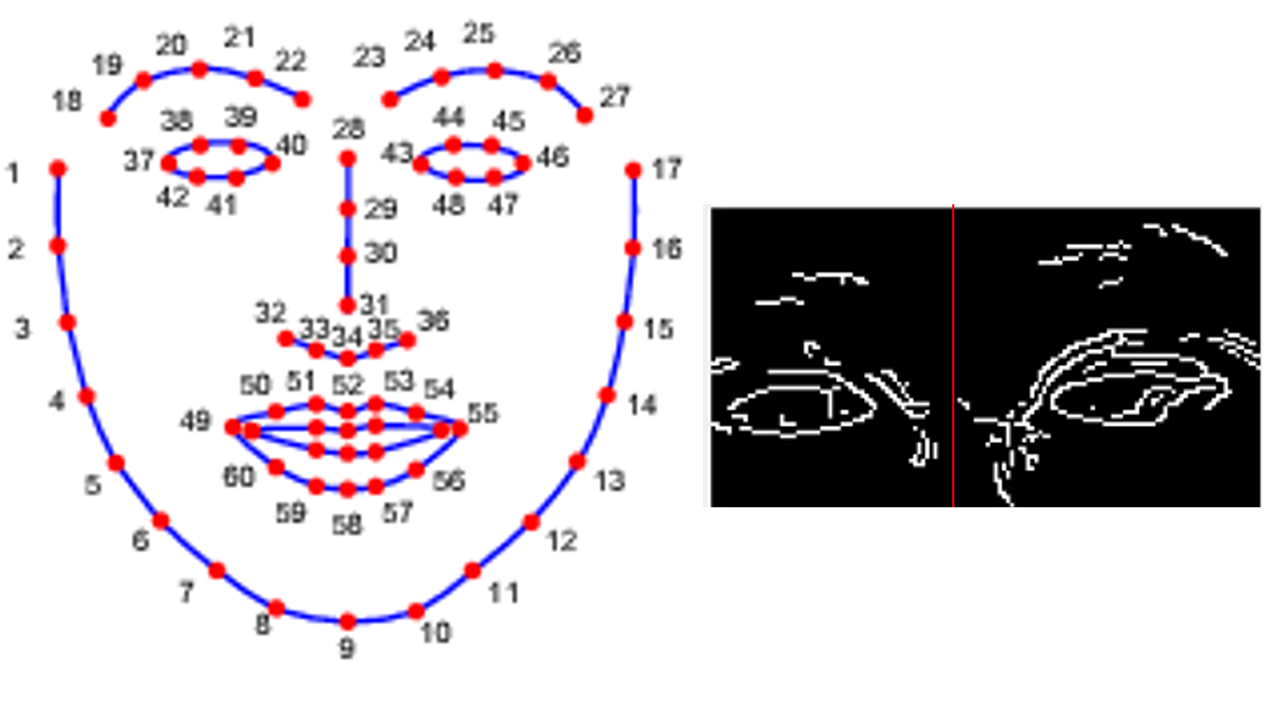
\includegraphics[width=6cm]{glasses-detection.png}\
        \caption{Using Edge Detection to Detect Glasses\label{glasses-detection}} 
    \end{center}
\end{figure}


\begin{figure}[tbh]
    \begin{center}
        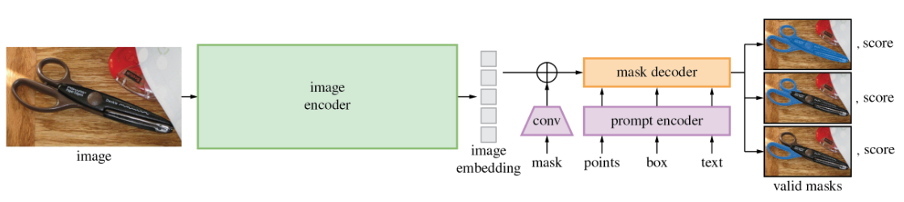
\includegraphics[width=8.5cm]{sam.png}\
        \caption{Segment Anything Model\label{figure2}} 
    \end{center}
\end{figure}

In order to determine if a person is holding an occluder over their eyes, object detection was required to identify the presence of the occluder. Due to the relatively small size of our dataset, we opted for transfer learning instead of training the model from scratch.

We selected YOLOv5 as the convolutional neural network (CNN) backbone. YOLOv5 belongs to the You Only Look Once (YOLO) \cite{redmon2016yolo} family of computer vision models and was released by Ultralytics in 2020. YOLOv5 offers four main versions: small (s), medium (m), large (l), and extra-large (x), each providing progressively higher accuracy rates but requiring varying amounts of training time \cite{ultralytics_yolov5}.

To begin, we utilized an online image annotator called Roboflow \cite{roboflow}, to perform image annotation. The images were annotated with labels such as \textit{RE\_occluder}, \textit{LE\_occluder}, \textit{RE\_occluder\_PH}, and \textit{LE\_occluder\_PH} (Figure \ref{figure7}). Once the annotation process was completed, the labels were downloaded in YOLO's labeling format. 

The images were resized to a standard size of 640 x 640 pixels, which is the default size for YOLOv5. Subsequently, the dataset was divided into training and testing sets. Our initial training involved a new classifier specifically for the four classes, while keeping the remaining layers frozen. The training parameters were set as follows: batch size of 10, 30 epochs, and the yolov5s6 model was utilized. We chose yolov5s6 because it strikes a good balance between speed and accuracy. Notably, the yolov5s6 model includes an additional output layer designed for detecting larger objects. These models benefit greatly from training at higher resolutions, resulting in improved detection outcomes.

However, in our specific case, we encountered sub-optimal results. Despite our best efforts, fine-tuning the model proved to be challenging and ultimately unsuccessful. During the testing phase, the YOLOv5 object detector failed to accurately detect the occluder.

\begin{figure}[tbh]
    \begin{center}
        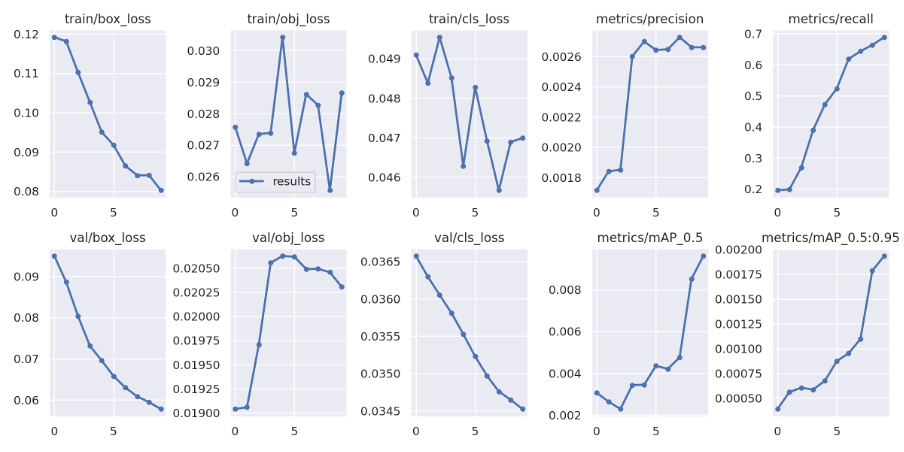
\includegraphics[width=8.5cm]{yolo_evaluation.png}\
        \caption{YOLOv5 evaluation metrics\label{yolo_evaluation}} 
    \end{center}
\end{figure}

\begin{figure}[tbh]
    \begin{center}
        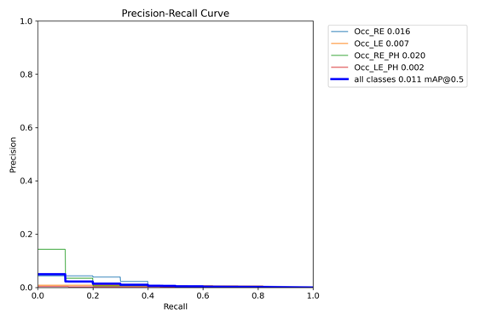
\includegraphics[width=8.5cm]{yolo_recall.png}\
        \caption{YOLOv5 Precision-Recall Curve\label{yolo_recall}} 
    \end{center}
\end{figure}

Next, we tried using the Segment Anything Model (SAM). Segment Anything Model, introduced by Meta in 2023, is a powerful tool for image segmentation. It can effectively segment images into masks without requiring additional training and exhibits impressive zero-shot performance across various segmentation tasks. Trained on the extensive SA-1B mask dataset, the model consists of a featurization transformer block and a decoder head that supports prompts. The model's architecture can be visualized using the diagram below.

We opted to leverage this model due to its outstanding segmentation capabilities. The usage of the model is straightforward. Following the installation of necessary dependencies and downloading the model's Git files, which include the weights, the SAM model is loaded into memory. We specifically chose the smallest ViT-B encoder to prioritize faster inference speed. To automatically generate masks, the \texttt{SAMAutomaticMaskGenerator} function is employed. This function returns a list of masks, with each mask represented as a dictionary containing various information pertaining to the mask.

Our objective is to create a dataset consisting of occluder and non-occluder masks. This dataset will be utilized for a subsequent SVM classifier to determine the orientations of occluders. Once the masks are generated, we iterate through each mask and save them accordingly.

While this method proves effective, we encountered a limitation when applying this approach to videos. It became evident that SAM's processing speed is insufficient for real-time video detection. The generation of masks for each frame takes several seconds, resulting in a delay in displaying the classification results in the video.

Nevertheless, we used the segmentation masks generated by the SAM model and trained a multi-class SVM classifier. Through confusion matrix evaluation, we observed that the classifier excelled in effectively distinguishing between different classes, yielding an impressive accuracy rate of 99.9\% (Figure \ref{confusion-matrix}). This outcome showcases the efficacy and reliability of our approach in achieving highly accurate and precise classification results.

To address the limitation of slow processing speed, we opted to utilize a thresholding method for generating segmentation masks in real-time processing. By incorporating the thresholding approach with SVM, we were able to achieve a processing speed of approximately 40 to 50 frames per second, facilitating real-time video analysis. However, we observed that the accuracy did not match our expectations in the final implementation.

This discrepancy in accuracy can be attributed to the inherent noise and reduced precision of the segmentation masks created through the thresholding method, as compared to the masks generated using SAM. Unfortunately, due to time and resource constraints, it was not feasible for us to create a new set of masks for training purposes. As a result, we focused on fine-tuning the hyperparameters for the threshold to optimize both accuracy and prediction stability.

Though we faced challenges in achieving the desired accuracy, we made the most of the available resources and implemented a solution that provided real-time video analysis.

\begin{figure}[tbh]
    \begin{center}
        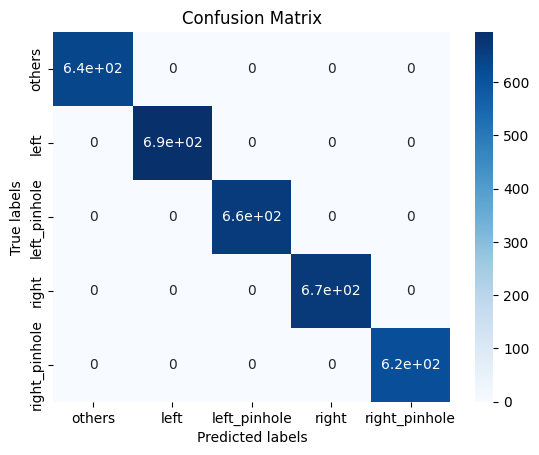
\includegraphics[width=8cm]{confusion_matrix_occuluder.png}\
        \caption{Confusion Matrix of SVM classifier for action recongnition\label{confusion-matrix}} 
    \end{center}
\end{figure}

\subsection{Discussions and limitations}
In this project, our primary objective was to develop a robust and comprehensive vision intelligent system capable of automating patient monitoring in the eye clinic. Our system encompasses multiple functionalities, including the ability to detect and extract identity information from an image of an identification card, detect and analyze portrait images, and perform face recognition for patient identification.

Throughout our development process, we conducted comprehensive evaluations of various approaches for feature extraction. Amongst the different feature extraction models, VGGFace emerged as the top performer, demonstrating superior performance in our evaluations.

However, during deployment, we encountered a significant limitation with our model. It became evident that the portraits extracted from the identity cards often differed greatly from the real-world appearance of the individuals. Most facial recognition systems rely on images captured directly from a person's face, incorporating various angles to gather an ample amount of facial features for robust reidentification. Without a suitable data augmentation technique, relying solely on a single portrait image for effective person reidentification can be an exceptionally challenging task.

The discrepancy between the identity card portraits and real-world appearances poses a significant obstacle to accurate and reliable recognition. 

To ensure that our system is not only accurate but also capable of real-time analysis, we made careful considerations in selecting computation-efficient methods. For instance, we leveraged the well-established Haar-Cascade classifier for efficient person detection. Additionally, we employed the canny edge detection technique to effectively identify the presence or absence of glasses.

To facilitate scene understanding and action detection, we adopted a single-frame analysis approach, utilizing image segmentation masks classified by a support vector machine (SVM) classifier. Initially, our intention was to employ the Segment Anything Model (SAM) for real-time image segmentation. However, during testing, we encountered significant delays in generating masks for a single frame. Despite our attempts to optimize performance by reducing image size or cropping, these efforts proved ineffective. Generating masks for each frame required a minimum of 10 seconds, falling short of the real-time analysis requirement of 20 to 30 frames per second. Consequently, we had to pivot to an alternative approach utilizing a simple thresholding method for mask creation.

While we achieved reasonably accurate predictions through hyperparameter adjustments, masks created via thresholding were inadequate for distinguishing between classes with subtle differences (e.g., "left" versus "left\_pinhole"). This limitation arises from the fact that masks generated using the thresholding method contain significant noise and lack the precision offered by the SAM model.

Despite the challenges faced, we made the necessary adjustments to ensure some level of accuracy in our predictions. However, it is important to acknowledge that the precision and distinction provided by the SAM model's masks were not fully replicated using the threshold approach. 

\section{Conclusions and future work}
In summary, we have developed a vision intelligent software solution capable of performing facial recognition, person detection, and recognition of patient actions. However, the current state of our solution is limited to a very specific and controlled environment. 

To enhance its performance, future efforts should focus on the redesign of the patient registration workflow, enabling the collection of more facial features for a more robust person re-identification process. 

Additionally, the current approach of using a single frame combined with image segmentation for scene understanding is suboptimal. To address this, future work should concentrate on creating a comprehensive training dataset and utilizing computational efficient segmentation techniques suitable for real-time analysis. Moreover, it would be beneficial to explore other real-time video analysis techniques, such as multi-frame analysis, to further improve the system's capabilities.

\section{Author contributions}
The authors confirm contribution to the paper as follows:
\begin{itemize}
\item \textbf{Lim Chang Siang}, conceptualized, literature review, system design, draft manuscript, experiment, system implementation and integration, performance evaluation and analysis, person recognition system, scene understanding system.
\item \textbf{Li Zhenghao, Kelvin}, conceptualized, literature review, product requirement specification, draft manuscript, data collection, domain expertise, scene understanding system, performance evaluation.
\item \textbf{Zhong Xiaohui}, conceptualized, requirement analysis, product requirement specification, system design, draft manuscript, experiment, person detection system.
\item \textbf{Zheng Xiaolan}, system design, draft manuscript, literature review, experiment, implementation, performance evaluation and analysis, scene understanding system.
\end{itemize}

All authors reviewed the results and approved the final version of the manuscript. 

The authors confirms sole responsibility for the following: solution conception and design, data collection, analysis and interpretation of results, and manuscript preparation.

\bibliographystyle{IEEEbib}
\bibliography{references}

\end{document}
